%\section{Calibration Hardware Overview}
%\label{sec:sp-calib-ov}

%\todo{Tables and figures seem to be shifted outside the sections and some not showing up. This needs Anne or other expert help...}
%\todo{SG: it seems that if you include \todo comments inside a table, it completely messes up the rest of the document. I tested this and once you remove those, figures and tables start showing up. Weird! But, now everything is in order.}
%%%%%%%%%%%%%%%%%%%%%%%%%%%%
\subsection{Introduction}
\label{sec:sp-calib-ov-intro}

\fixme{(from Nora) I must point out that the headings in this document are problematic. They go to five levels, in some places (see page 7 on the PDF) with no text until the fifth level heading. This is extremely troubling. Generally, no heading should appear without at least transitional text following it, and here we have three headings with nothing, no content, no transitions, no indications of anything. This will not do. This is especially troublesome later in the chapter when bold is used to designate sections without using headings at all (see page 8 of the PDF). I strongly advise cutting the levels of heading down to three and making sure that text follows each heading. Major headings could use introductory text for that section/chapter while most subheadings should have content following. If you look, you will note that you already have text that can be used for those purposes. For instance, Section 1.1.1 is an introduction to the entire chapter. Some portions of this introduction appear to go with Section 1.1, the overview of the first part. One way to handle this is to put all the headings into a separate file and find the information that goes with the headings. You can then copy and paste the text to the appropriate section with the appropriate heading. If the heading has no text, that heading would be eliminated or text would be provided. This gives you a visual of how the paper fits together. One final note: too many headings cause confusion. (Too few headings also cause confusion.)}

%% Connection to Physics chapter-- Idea of calibration strategy.
%% Describe here the design and systems we plan to deploy
A detailed understanding of the overall detector response is essential for DUNE physics goals. The precision with which each calibration parameter needs to be measured is set by the systematic uncertainties for the \dword{lbl} and other physics programs at DUNE. Chapter~4 of the Physics volume of the TDR provides a detailed description of the calibration strategy for the DUNE FD using existing sources of particles (e.g. cosmic ray muons), external measurements (e.g. ProtoDUNE), monitors (e.g. purity monitors) and dedicated calibration hardware systems. 

This chapter describes the dedicated calibration systems, to be deployed for the DUNE \spmod which are intended to provide necessary information beyond the reach of external measurements and existing sources and monitors. These include an ionization laser system, a photoelectron laser system and a pulsed neutron source system. The possibility of deploying a radioactive source system is also currently being explored.  
%This chapter describes the design of the dedicated calibration systems to be deployed for the DUNE \spmod.  As discussed in the Physics TDR\fixme{proper reference}, the calibration strategy includes external measurements (e.g. ProtoDUNE), monitors (e.g. purity, thermal), existing sources of particles (e.g. muons from cosmic rays), and dedicated external calibration hardware systems.  This chapter discusses the calibration hardware systems. Monitoring systems are discussed in other chapters: CISC (purity, thermal monitors, slow control), PDS (LED stability system\fixme{proper name is?}), and CE (charge injection system). The physics TDR discusses the use of existing sources of particles, and external measurements. 

Section~\ref{sec:sp-calib-ov-scope} describes the baseline hardware designs, and outlines alternative designs which may improve physics capability and/or reduce overall cost. Section~\ref{sec:sp-calib-sys-las} describes the baseline design for the ionization laser system, which provides an independent, fine-grained measurement of the electric field throughout the detector which is an essential parameter that impacts the spatial and energy resolution of physics signals. Such a system also offers many secondary uses such as alignment checks, stability monitoring, and diagnosing detector failures.
Section~\ref{sec:sp-calib-sys-las-pe} describes the photoelectron laser system which can be used to rapidly diagnose electronics or TPC response issues along with many other useful measurements such as integrated field across drift, drift velocity, and electronics gain. Section~\ref{sec:sp-calib-sys-pns} describes the baseline design for the pulsed neutron source, which provides a triggered, well defined energy deposition from neutron capture in Ar detectable throughout the detector volume. Neutron capture forms a critical component of signal processes for \dword{snb} and \dword{lbl} physics enabling direct testing of the detector response spatially and temporally for the low-energy program. The proposed radioactive source system, which is complementary to the pulsed neutron source system, provides an in-situ source of gamma rays in the same energy range of
\dword{snb} and solar neutrino physics, and is described in Section~\ref{sec:sp-calib-sys-rs}. 

The DAQ requirements for calibration sources and systems are described in Section~\ref{sec:sp-calib-daqreq}. For all the calibration hardware systems, the goal is deploy prototype designs and validate them at ProtoDUNE as part of the post long shutdown 2 (LS2) running  at CERN. The validation plan envisioned for calibration systems at ProtoDUNE and other experiments is described in Section~\ref{sec:sp-calib-val}. The Calibration Consortium was formed in November 2018. As such, significant development plans exist and the timeline for these is outlined in Section~\ref{sec:sp-calib-sched}.
%A large part of the work done so far has been done within the Calibration Task Force; 

%%%%%%%%%%%%%%%%%%%%%%%%%%%%
\subsection{Scope}
\label{sec:sp-calib-ov-scope}
% KM outline
%% Scope is: baseline designs for Laser system and neutron system.
%% Alternative designs, including additional capabilities of the laser system, radioactive source are considered.

%%calibration review in May. "what's the scope? How many lasers we need? How many ports needed? Do we need crossing tracks? do we need to penetrate FC ? what does the HV consortium think about that?"

The scope of the calibration consortium includes a laser ionization system, a photoelectron laser system, a laser positioning system, a pulsed neutron source system. In addition, the consortium is evaluating the possibility of a radioactive source system. The calibration consortium is responsible for design through commissioning in the SP module for these calibration devices and their associated feedthroughs. Validating the designs of calibration systems at ProtoDUNE (and other experiments as relevant) is also included under the scope of the consortium. Figure~\ref{fig:scope_chart} shows the subsystems included under the calibration consortium. 

Chapters 3, 4, 5 and 8 describe other hardware that are essential for calibration such as \dword{ce} external charge injection systems, \dword{hv} monitoring devices, PDS,
stability monitoring system, and cryogenic instrumentation and detector monitoring devices, respectively. The scope of these systems are included in their respective consortia and the calibration consortium has substantial interfaces with them. 

The usage of other calibration sources such as external measurements, and existing sources of particles (e.g. muons, pions) is discussed in the physics volume of the TDR. The impact of calibration on physics and related studies are currently pursued under the calibration task force and the consortium works closely with the task force to make physics connections. Calibrations also require significant simulation work such as E field simulations to identify desirable locations for instrumentation devices in the cryostat, away from regions of high E field, so that their presence does not induce large field distortions. 

%Calibration has additional activities outside the scope of the consortium that require coordination with other groups. This is discussed in Section~\ref{sec:sp-calib-intfc}. 
The design of the calibration systems and understanding related physics requires coordination with other consortium and groups. This is discussed in Section~\ref{sec:sp-calib-intfc}, which also includes necessary tools (e.g. physics simulations) developed in conjunction with the physics groups (and calibration task force).

\begin{figure}[tbp]
\centering
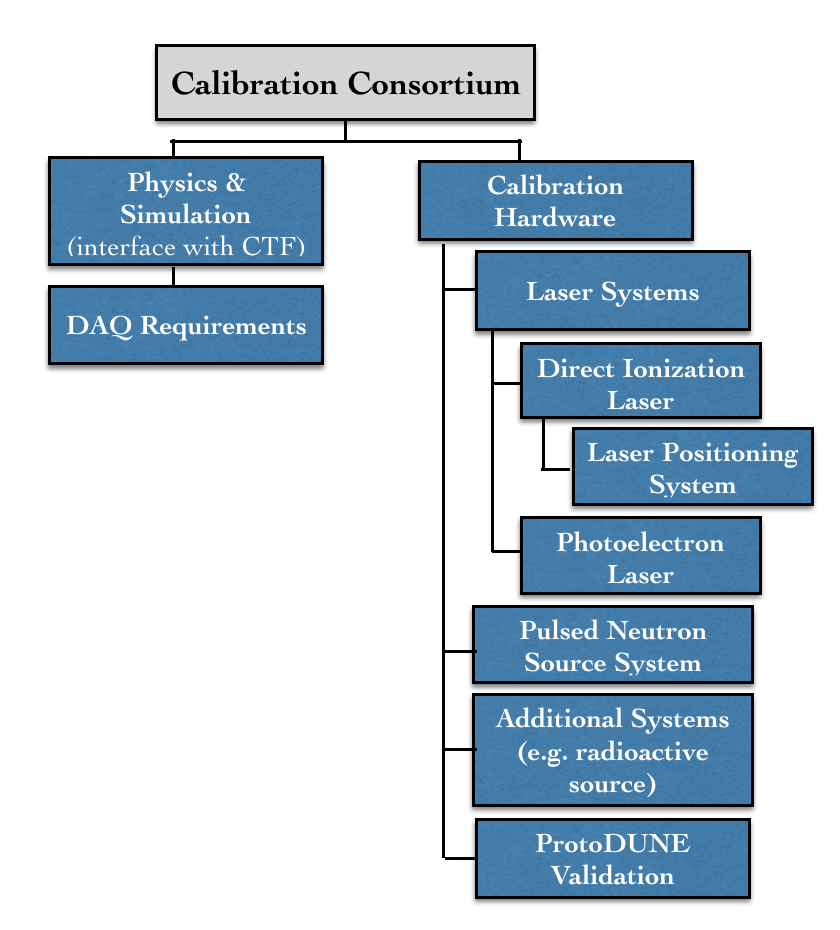
\includegraphics[height=4.0in]{graphics/calib_scope_chart.png}
\caption{Calibration consortium subsystem chart.}
\label{fig:scope_chart}
\end{figure}

%%%%%%%%%%%%%%%%%%%%%%%%%%%%
%\subsection{Requirements}
%\label{sec:sp-calib-ov-req}

%\input{vol-sp/ch-sp-calib-requirements}


%%%%%%%%%%%%%%%%%%%%%%%%%%%%
\subsection{Design Considerations and Requirements}
\label{sec:sp-calib-ov-consid}
%\fixme{SG, KM: Done; JM please check. }
%To-DO: Need more information on requirements from neutron source and RA source, once we have it, we can update the text/table as needed.}

Some common design considerations for calibration devices include stability, reliability, and longevity, so that calibration systems can be operated for the lifetime of the experiment (\dunelifetime). Such longevity is uncommon for any device, so the overall design allows replacement of devices where possible. The systems must also adhere to relevant global requirements of the DUNE detector; Table~\ref{tab:fdgen-calib-toplevel-reqs} shows the top-level requirements for calibration subsystems from the overall requirements. For example, DUNE requires the \efield  on any instrumentation devices inside the cryostat to be less than 30 kV/cm to minimize the risk of dielectric breakdown in \lar. A consideration important for event reconstruction is the maximum noise level induced by calibration devices that the readout electronics can tolerate. \dword{pdsp} is evaluating this. 

Table~\ref{tab:fdgen-calib-toplevel-reqs} \todo{This table was prepared manually not automatically generated; But, we have prepared the appropriate spreadsheet.} also shows the top-level requirements from each calibration subsystem. For the laser system, the energy and position reconstruction requirements for physics measurements lead to requirements on the necessary precision of the laser \efield measurement, its spatial coverage and granularity. The laser \efield measurement precision is required to be ~1\% so that the impact on the collected charge is well below 1\%. This is also motivated by consistency with the high level DUNE specification of 1\% on field uniformity throughout the volume due to component alignment and \hv system. For the laser coverage, in order to keep the \efield measurement precision at the ~1\% level, we aim to have a coverage of 75\% or better of the total fiducial volume (FV). The requirement on the granularity for laser is estimated based on the FV uncertainty requirements (1\%) and corresponding uncertainty requirements (1.5 cm) in each coordinate. A voxel size of \num{30}x\num{30}x\num{30}~cm is considered to be sufficient to satisfy the FV uncertainty requirements. 

The laser beam position is also required at the level of reconstruction requirement in each coordinate which is around 5~mm over 10 to 15~m where the latter is the distance between two consecutive laser ports in the beam direction. This results in a stringent requirement of 0.03$^{o}$ (or 0.5~mrad). The data volume for the ionization laser system is required to be at least 90~TB/year/10-kton assuming 800k laser pulses, \num{10}x\num{10}x\num{10}~cm voxel sizes, a 100~$\mu$s zero suppression window, and one dedicated calibration campaign per year.

For the pulsed neutron source system, the system must provide sufficient neutron event rate to make spatially separated precision measurements across the detector of comparable size to the voxels probed by the laser (\num{30}x\num{30}x\num{30}~cm) for most regions of the detector (75\%). For the supernova program, measurements from the PNS should demonstrate 1\% energy scale, 5\% energy resolution and 0.5 MeV detection threshold, and so each voxel should have sufficient neutron event rate to achieve this. %\todo{KM: Improve or remind connection to SN program? even though it's comparable? SG: maybe for 2nd draft?}
In terms of data volume requirements, the neutron source system requires about 84~TB/year/10-kton assuming 10$^{6}$ neutrons/pulse, 1000 neutron captures/m$^{3}$ and 1300 observed neutron captures per pulse and 6 calibration runs per year. 

For the proposed radioactive source system, it is important that the rate of the 9 MeV capture $\gamma$ events inside the source is less than 1~kHz so no more than one capture $\gamma$-event occurs during a single 2.2~ms drift period. 

Table~\ref{tab:fdgen-calib-all-reqs} shows the full set of requirements related to all of the calibration subsystems. More details on each of the requirements can be found under corresponding consortia.   
%\todo{Updated estimate for PNS DAQ rate to be added to Table 1.1 and 1.2}

\begin{dunetable}
[Specifications for calibration subsystems]
{p{0.45\linewidth}p{0.25\linewidth}p{0.25\linewidth}}
{tab:fdgen-calib-toplevel-reqs}
{List of top-level specifications for the different calibration subsystems. Global DUNE requirements are listed in bold.}  Quantity/Parameter	& Specification	& Goal		 \\ \toprowrule      
{\bf Noise from calibration devices}	 & $\ll$ 1000 enc   & \\ \colhline    
{\bf Max. \efield near calibration devices} & < 30 kV/cm & <15 kV/cm \\ \colhline     
Ionization Laser \efield measurement precision & 1\% & <1\% \\ \colhline
Ionization Laser \efield measurement coverage & > 75\% & 100\% \\ \colhline
Ionization Laser \efield measurement granularity & < \num{30}x\num{30}x\num{30}~cm & \num{10}x\num{10}x\num{10}~cm \\ \colhline
Laser beam position precision & 0.5 mrad & 0.5 mrad \\ \colhline
Neutron source coverage & > 75\% & 100\% \\ \colhline % neutron source
Ionization laser DAQ rate (per 10 kton) & 90~TB/year & 185~TB/year\\ \colhline
Neutron source DAQ rate (per 10~kton) & 84~TB/year & 168~TB/year\\ \colhline
Rate of 9~MeV capture $\gamma$-events inside the proposed radioactive source & < 1~kHz & \\ \colhline 
\end{dunetable}


\begin{dunetable}
[Specifications for calibration subsystems]
{p{0.45\linewidth}p{0.25\linewidth}p{0.25\linewidth}}
{tab:fdgen-calib-all-reqs}
{List of specifications for the different calibration subsystems}   
Quantity/Parameter	& Specification	& Goal		 \\ \toprowrule      

Noise from calibration devices	 & $\ll$ 1000 enc   & \\ \colhline    Max. \efield near calibration devices & < 30 kV/cm & <15 kV/cm \\ \colhline                     

\textbf{Direct Ionization Laser System} &    &   \\ \colhline   
\efield measurement precision & 1\% & <1\% \\ \colhline
\efield measurement coverage & > 75\% & 100\% \\ \colhline
\efield measurement granularity & < \num{30}x\num{30}x\num{30}~cm & \num{10}x\num{10}x\num{10}~cm \\ \colhline
Top field cage penetrations (alternative design) & to achieve desired laser coverage & \\ \colhline
DAQ rate per 10~kton & 90 TB/year & 185 TB/year \\ \colhline
Longevity	& \dunelifetime			& > \dunelifetime   \\ \colhline        
%Stability & Match precision requirement at all places/times	&  \\ \colhline  Reliability	& Measurements as needed & Measurements as needed \\ \colhline 
\textbf{Laser Positioning System} & & \\ \colhline                      
Laser beam position precision & 0.5~mrad & 0.5~mrad \\ \colhline
Longevity	& \dunelifetime			& > \dunelifetime   \\ \colhline        
%Stability & Match precision requirement at all places/times	&  \\ \colhline  Reliability	& Measurements as needed & Measurements as needed \\ \colhline    
\textbf{Photoelectron Laser System}	   &   &  \\ \colhline            
Longevity	& \dunelifetime			& > \dunelifetime   \\ \colhline        
%Stability & Match precision requirement at all places/times	&  \\ \colhline  Reliability	& Measurements as needed & Measurements as needed \\ \colhline

\textbf{Pulsed Neutron Source System}	   &   &  \\ \colhline        
Coverage & > 75\% & 100\% \\ \colhline
DAQ rate per 10~kton & 84~TB/year & 168~TB/year \\ \colhline 
Longevity	& 3 years			& \dunelifetime   \\ \colhline        
%Stability & Match precision requirement at all places/times	&  \\ 
%\colhline  Reliability	& Measurements as needed & Measurements as needed \\ \colhline

\textbf{Proposed Radioactive Source System}	   &   &  \\ \colhline  
Distance of the source from the field cage & 30 cm & \\ \colhline
Rate of 9~MeV capture $\gamma$-events inside the source & < 1kHz & \\ \colhline 
Data volume per 10~kton & 50~TB/year & 100~TB/year \\ \colhline 
Longevity	& \dunelifetime			& > \dunelifetime   \\ \colhline    
%Stability & Match precision requirement at all places/times	&  \\ \colhline  Reliability	& Measurements as needed & Measurements as needed \\ \colhline

\end{dunetable}


\subsubsection{Cryostat Configuration for Calibration}
\label{sec:calib-ports}
The current cryostat design for the %DUNE SP FD 
\spmod with penetrations for various sub-systems is shown in Figure~\ref{fig:ftmap}. The penetrations dedicated for calibrations are highlighted in black circles. The ports on far east and far west are located outside the field cage. The current plan is to use these penetrations for multiple purposes. For example, the penetrations on the far east and west will be used both by laser and radioactive source systems. In addition to these dedicated ports, the Detector Support System (DSS) and cryogenic ports (orange and blue dots in Figure~\ref{fig:ftmap}, respectively) will also be used as needed to route cables for calibration systems (e.g. the \dword{sp} \dword{pds}). There is plan to accommodate DSS and cryogenic ports with feedthroughs with a CF63 side flange for this purpose.   

\begin{figure}[tbp]
\centering
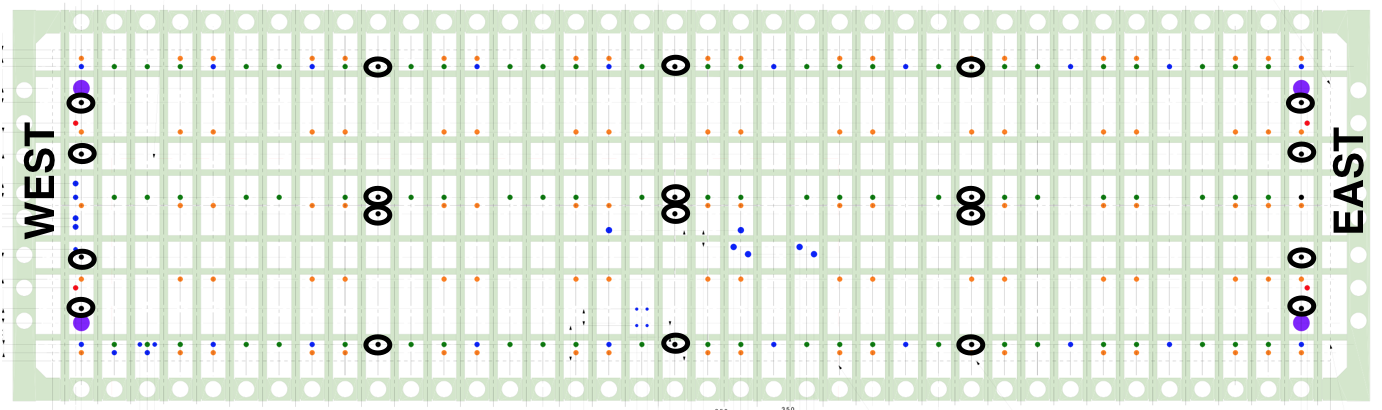
\includegraphics[height=2.0in]{FTmap.png}
\caption{Top view of the \spmod %DUNE SP FD 
cryostat showing various penetrations. Highlighted in black circles are multi-purpose calibration penetrations. The green dots are TPC signal cable penetrations. The blue ports are cryogenic ports. The orange ports are \dword{dss} penetrations. The larger purple ports at the four corners of the cryostat are human access ports.}
\label{fig:ftmap}
\end{figure}

The placement of these penetrations was largely driven by the ionization track laser %and radioactive source system 
requirements. The ports that are inwards of the cryostat are placed near the APAs (similarly to what is planned for SBND) to minimize any risks due to the HV discharge. For the far east and west ports, HV is not an issue as they are located outside the \dword{fc} and the penetrations are located near mid-drift (location favorable to possible source deployment).
%to meet radioactive source requirements. 
Implementation of the ionization track laser system proposed in Section~\ref{sec:sp-calib-sys-las-ion}, requires 20 feedthroughs to cover the four TPC drift volumes; this arrangement is needed for lasers to be used for full volume calibration of the E field and associated diagnostics (e.g. HV). 

The distance between any two consecutive feedthrough columns in Figure~\ref{fig:ftmap} is assumed to be about \SI{15}{\m}. This is considered reasonable since the experience from the \microboone laser system has shown that tracks will propagate over that detector's full \SI{10}{\m} length. Assuming that the effects of Rayleigh scattering and self-focusing (Kerr effect) do not limit the laser track length, this laser arrangement could illuminate the full volume with crossing track data.  It is important to note that at this point in time, a maximum usable track length is unknown and it is not excluded that the full \SI{60}{\m} \detmodule length could be achieved by the laser system after optimization.


